\documentclass[UTF8,11pt]{ctexart}
\usepackage[a4paper,margin=2.2cm]{geometry}
\usepackage{graphicx}
\usepackage{subcaption}
\usepackage{booktabs}
\usepackage{amsmath}
\usepackage{siunitx}
\usepackage{xcolor}
\usepackage{hyperref}

\hypersetup{colorlinks=true,linkcolor=blue,citecolor=blue,urlcolor=blue}
\sisetup{detect-all=true}

\title{表面活性剂调控薄膜缺陷与表观力学性能}
\author{}
\date{}

\begin{document}
\maketitle

\section{表面活性剂、缺陷结构与深压入力学性能}

为避免接近段吸附、回撤粘附和限域水桥对力学参数的混淆，本节仅分析 RealRaw 数据中深压入 extend/loading 分支的正力加载段。原始曲线经接触点识别和悬臂梁顺应性校正后，将可恢复的 stick--slip 滑脱事件通过垂直力偏移拼接为连续加载曲线；原始力值保留为 \texttt{raw\_force}，拼接后的 \texttt{stitched\_force} 仅作为力学拟合视图。末端不可恢复的悬崖式掉落不参与拟合。因此，下文所有模量均定义为模型依赖的表观膜模量（model-dependent apparent Young's modulus），用于同一探针和同一数据集内部的相对比较，而不直接等同于材料本征 Young's modulus。

深压入曲线采用圆形夹持悬膜的经验加载模型：
\begin{equation}
    F = k_1 \delta + k_3 \delta^3 ,
    \label{eq:membrane-fit}
\end{equation}
其中 $F$ 为加载力，$\delta$ 为悬臂梁校正后的压入深度，$k_1$ 代表低压入区的线性张力/接触刚度贡献，$k_3$ 代表大变形拉伸主导的非线性膜响应。依据 AFM 悬膜压入常用形式，将 cubic 项换算为表观三维模量：
\begin{equation}
    E_{\mathrm{app}} = \frac{k_3 a^2}{q^3 t},
    \qquad
    q = \frac{1}{1.05 - 0.15\nu - 0.16\nu^2}.
    \label{eq:eapp}
\end{equation}
本文默认孔半径 $a=\SI{10}{\micro\meter}$，泊松比 $\nu=0.30$，主膜厚 $t=\SI{50}{\nano\meter}$，并给出 $t=\SI{80}{\nano\meter}$ 时的敏感性估计。由于 $E_{\mathrm{app}}\propto 1/t$，膜厚不确定性会线性传递到模量绝对值。对于线性项，还计算表观膜张力
\begin{equation}
    T_{\mathrm{app}} = \frac{k_1\ln(a/r_{\mathrm{tip}})}{2\pi},
    \qquad
    \sigma_{\mathrm{app}} = \frac{T_{\mathrm{app}}}{t},
    \label{eq:tension}
\end{equation}
但 $T_{\mathrm{app}}$ 和 $\sigma_{\mathrm{app}}$ 仅作为比较性参数使用。

\begin{figure}[htbp]
    \centering
    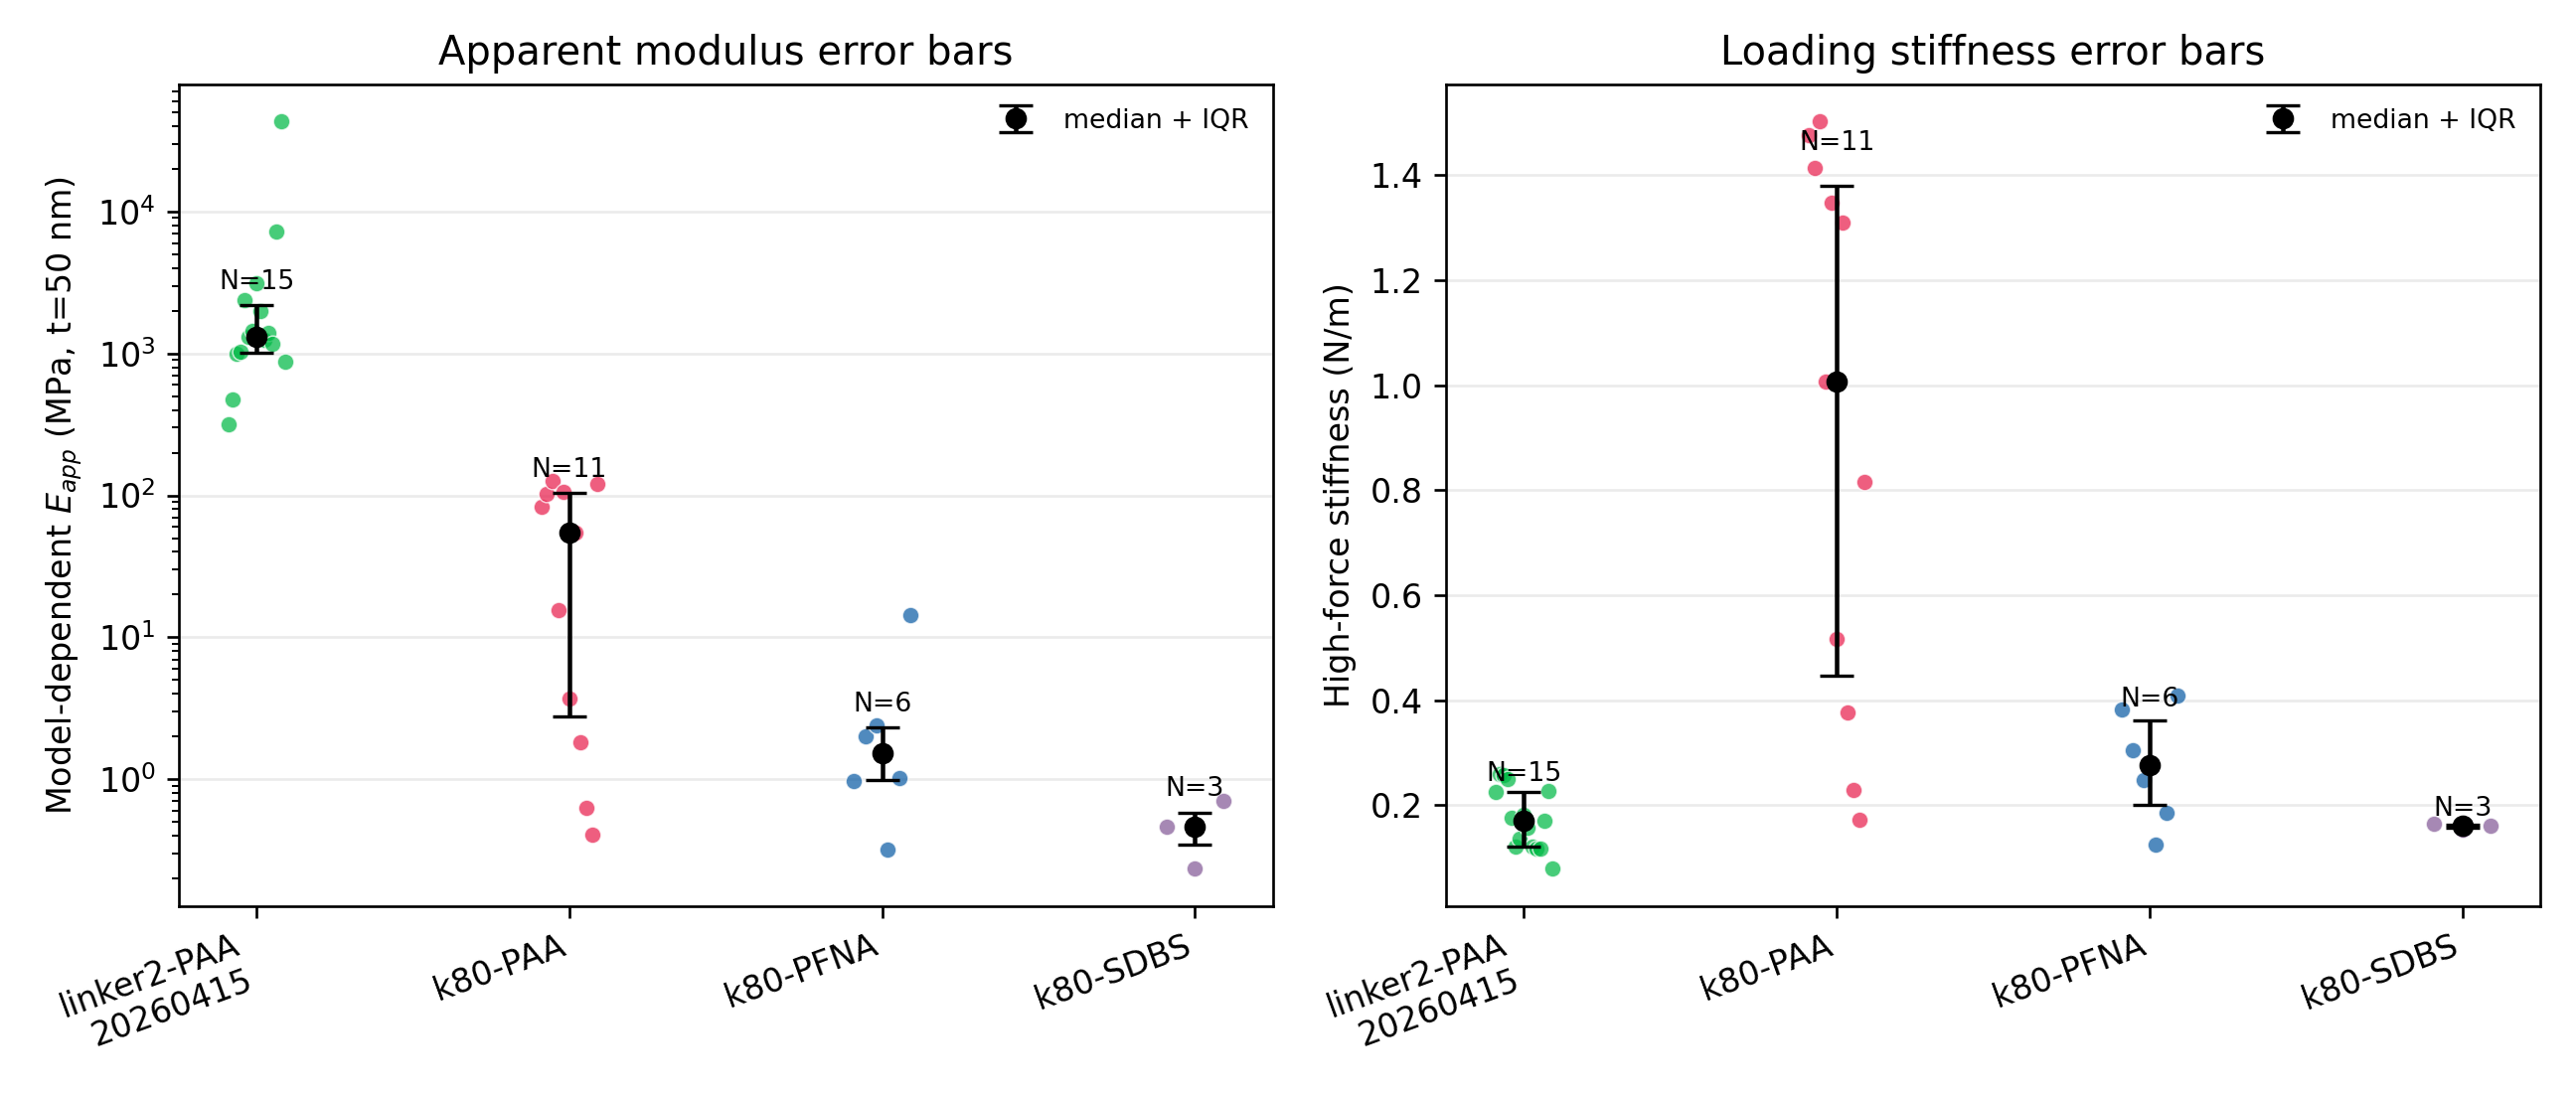
\includegraphics[width=0.96\linewidth]{median_iqr_errorbars.png}
    \caption{深压入 apparent modulus 和高力区刚度的误差棒统计。散点表示每条有效 force curve，黑色中心点表示中位数，误差棒表示四分位范围（Q1--Q3）。这种 median+IQR 表示方式避免了少数高 $k_3$ 曲线对均值和 SEM 的过度拉高。}
    \label{fig:median-iqr}
\end{figure}

\begin{figure}[htbp]
    \centering
    \begin{subfigure}[t]{0.48\linewidth}
        \centering
        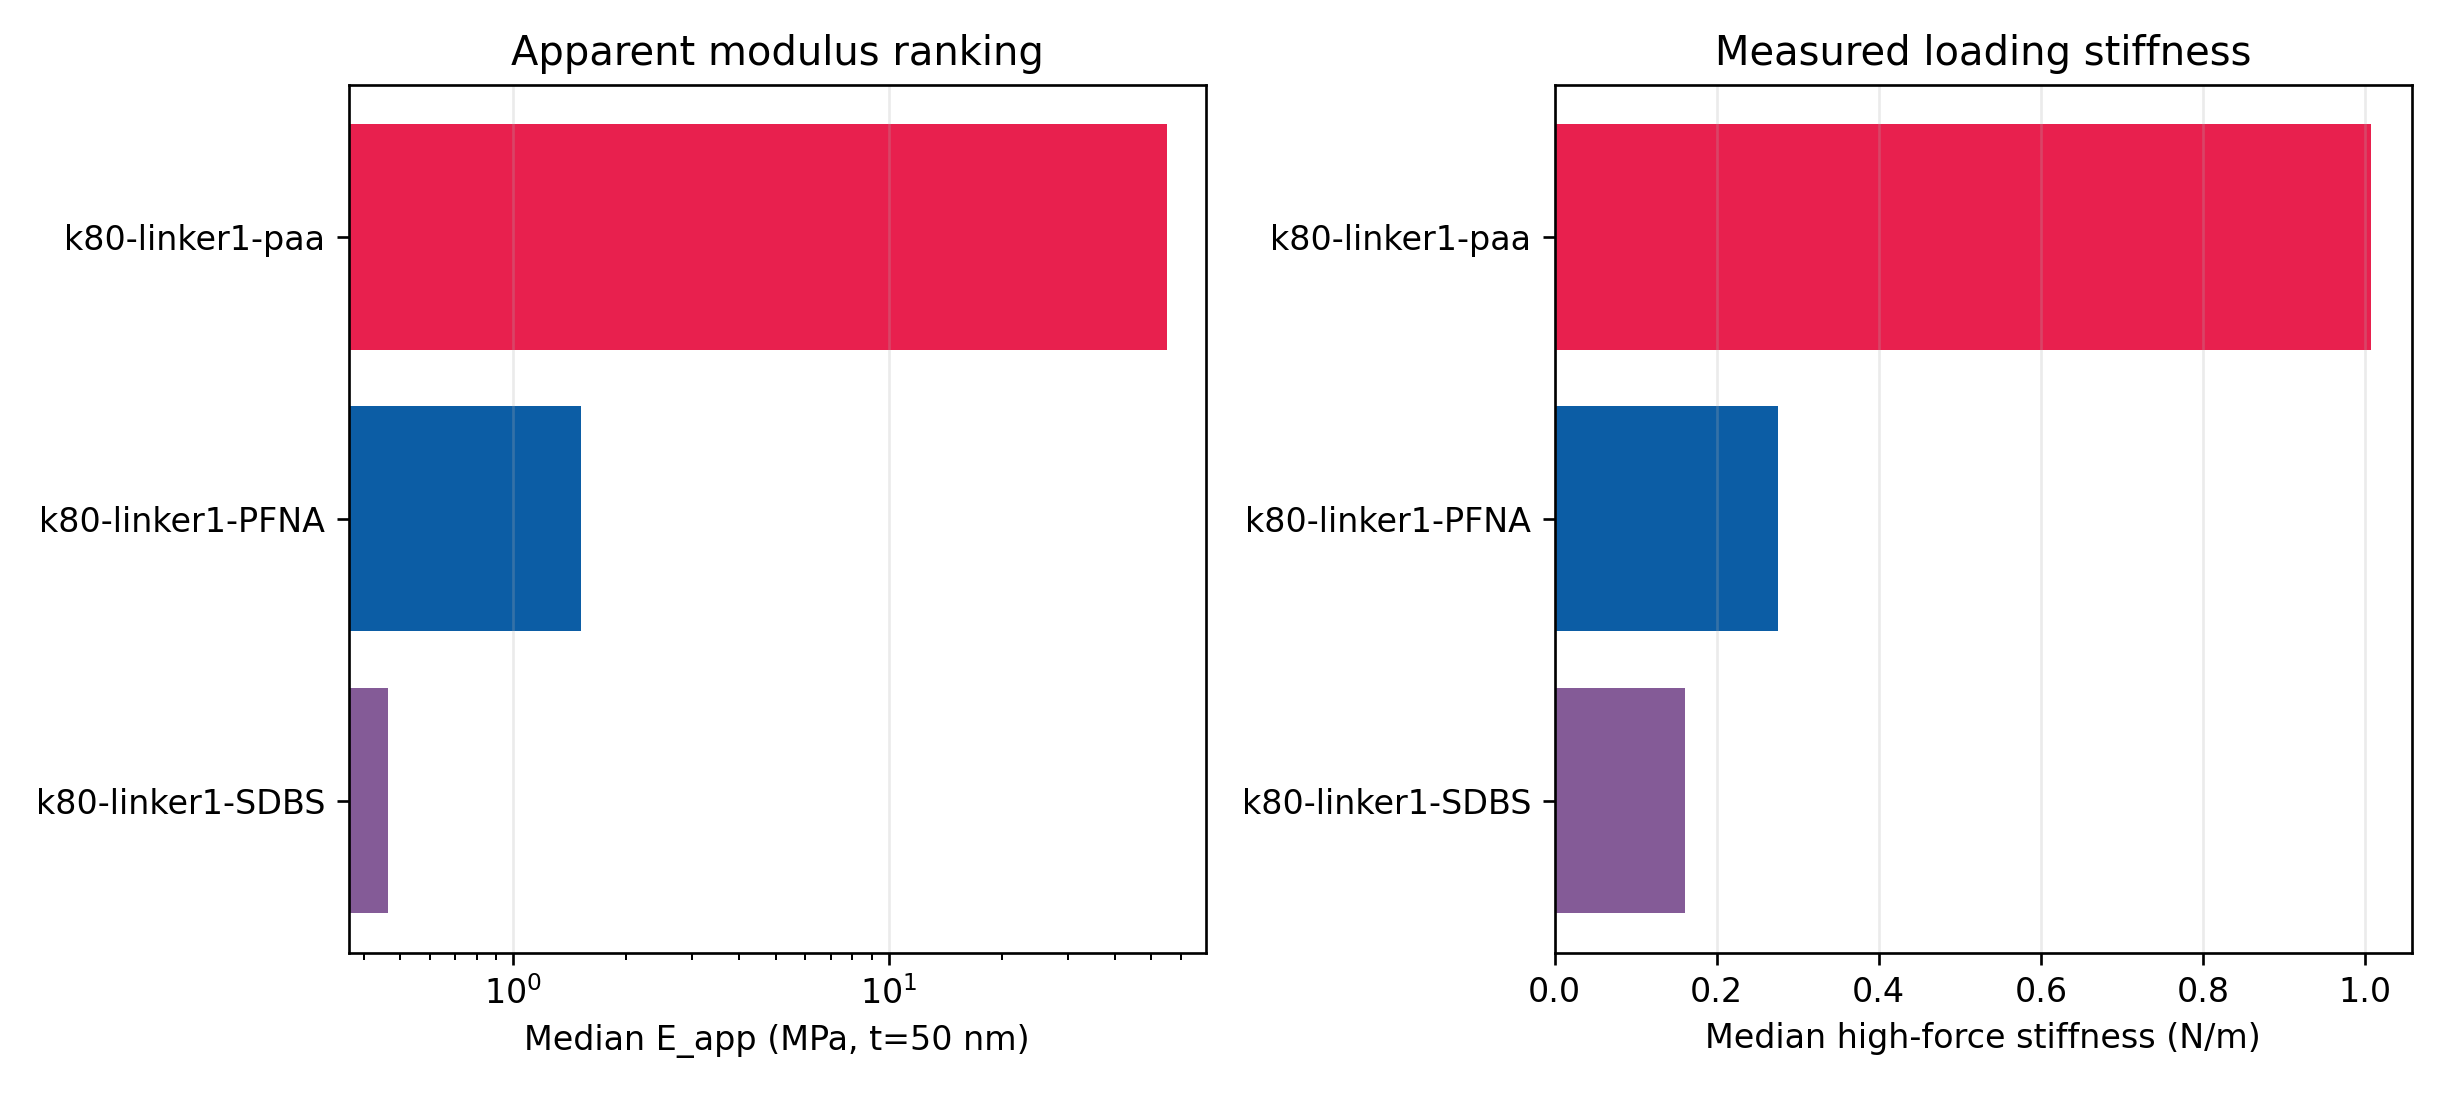
\includegraphics[width=\linewidth]{surfactant_mechanics_ranking.png}
        \caption{基于深压入曲线的 k80 表面活性剂力学排序。}
        \label{fig:ranking}
    \end{subfigure}
    \hfill
    \begin{subfigure}[t]{0.48\linewidth}
        \centering
        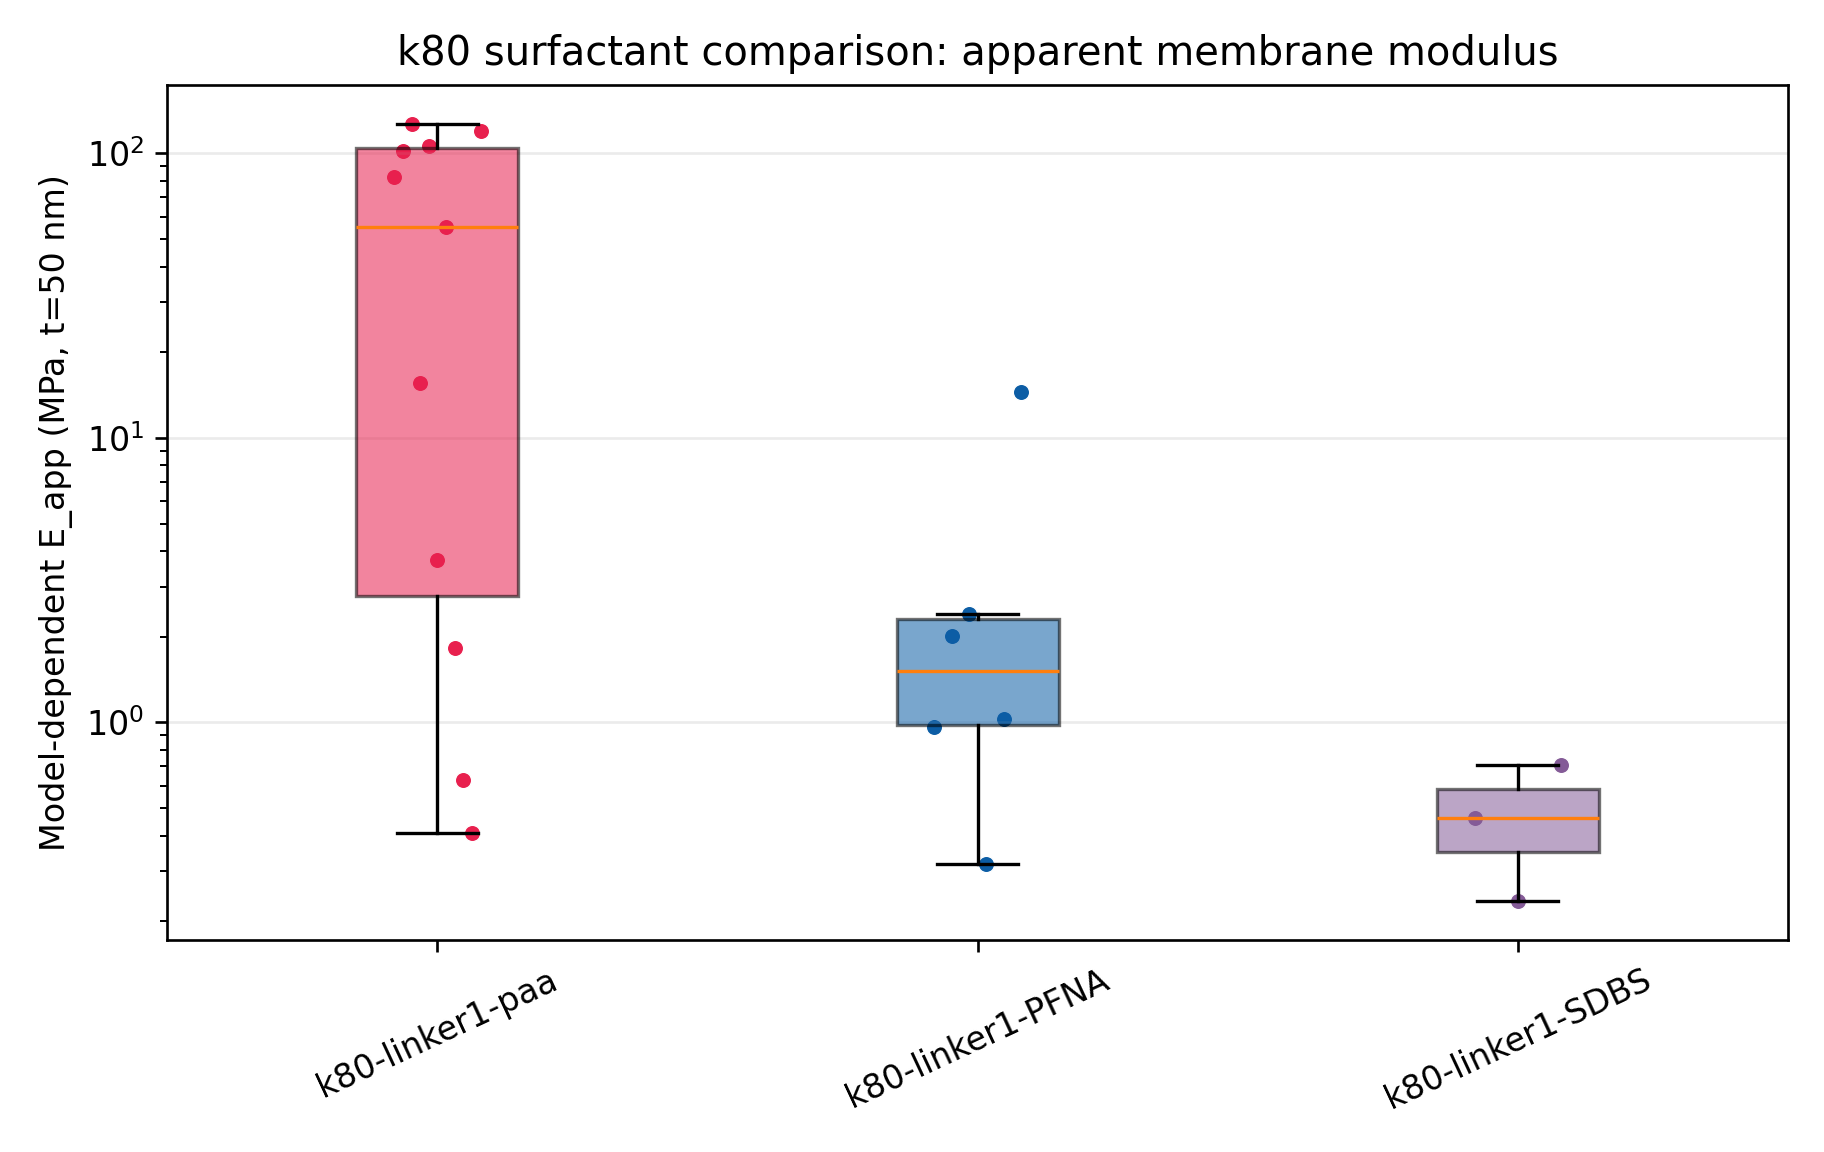
\includegraphics[width=\linewidth]{k80_surfactant_Eapp_boxplot.png}
        \caption{20260416 k80 系列的 $E_{\mathrm{app}}$ 分布。}
        \label{fig:boxplot}
    \end{subfigure}
    \vspace{0.5em}
    \begin{subfigure}[t]{0.48\linewidth}
        \centering
        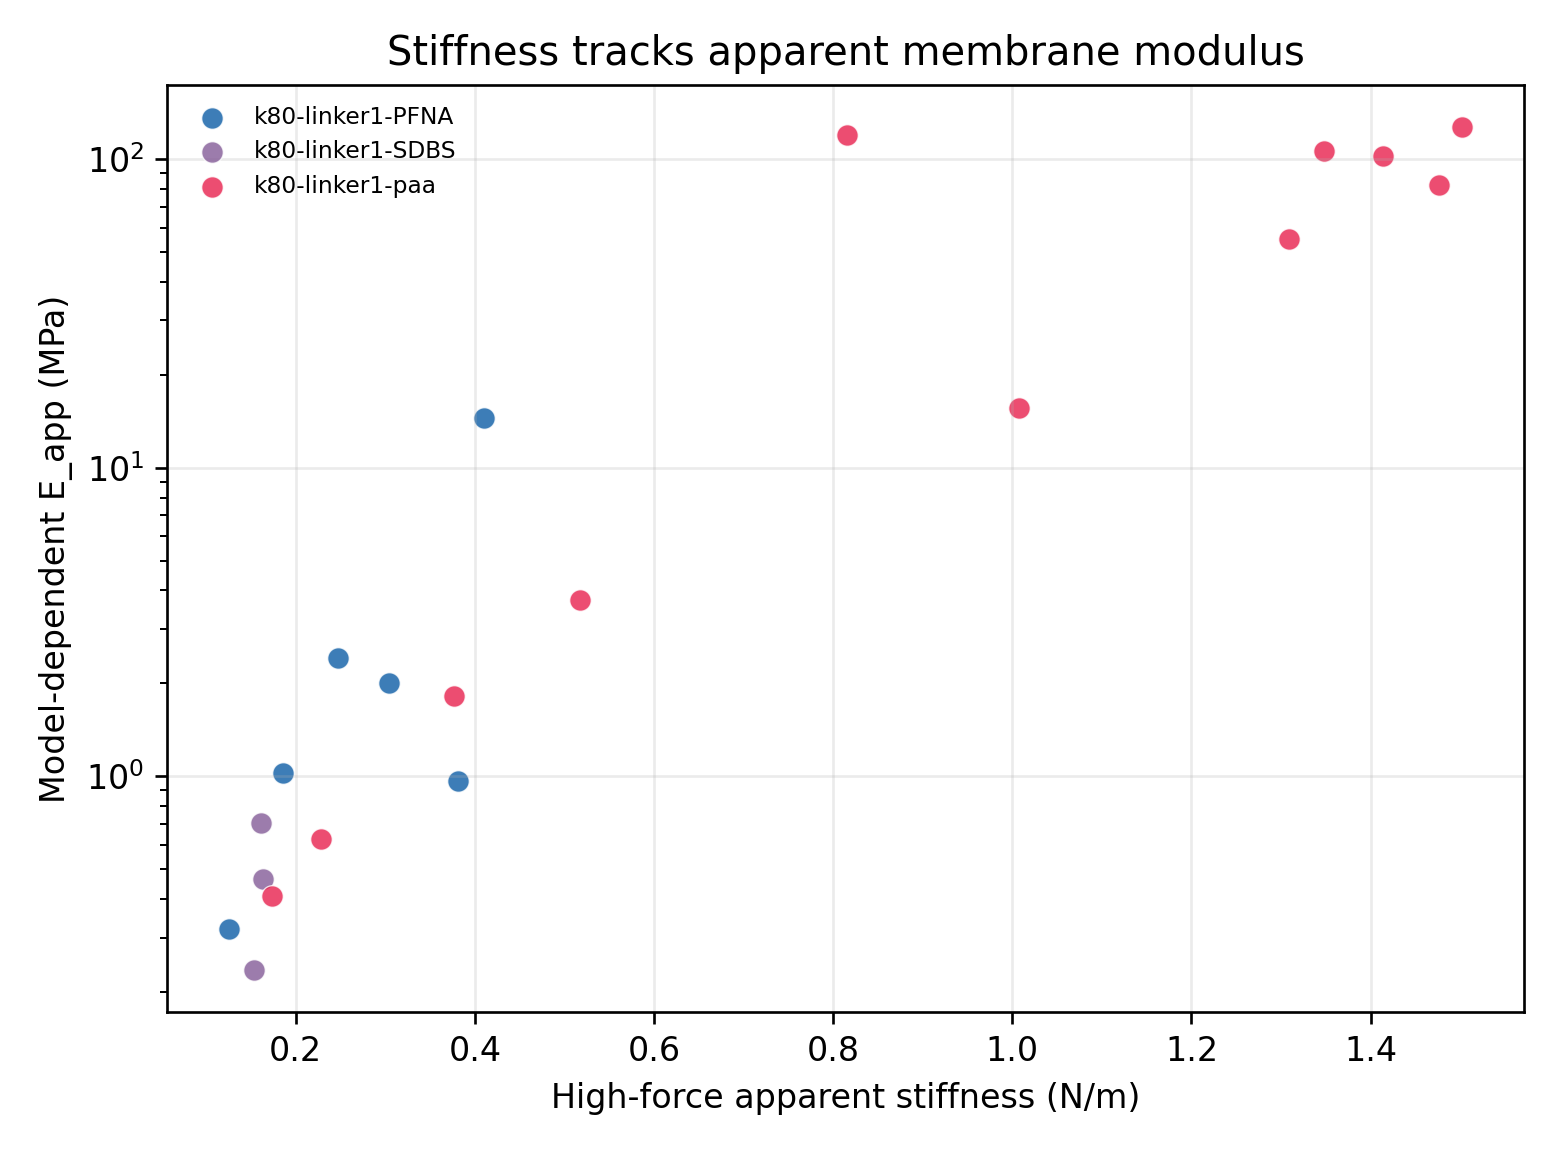
\includegraphics[width=\linewidth]{k80_surfactant_stiffness_vs_Eapp.png}
        \caption{高力区刚度与 $E_{\mathrm{app}}$ 的对应关系。}
        \label{fig:stiffness-vs-e}
    \end{subfigure}
    \hfill
    \begin{subfigure}[t]{0.48\linewidth}
        \centering
        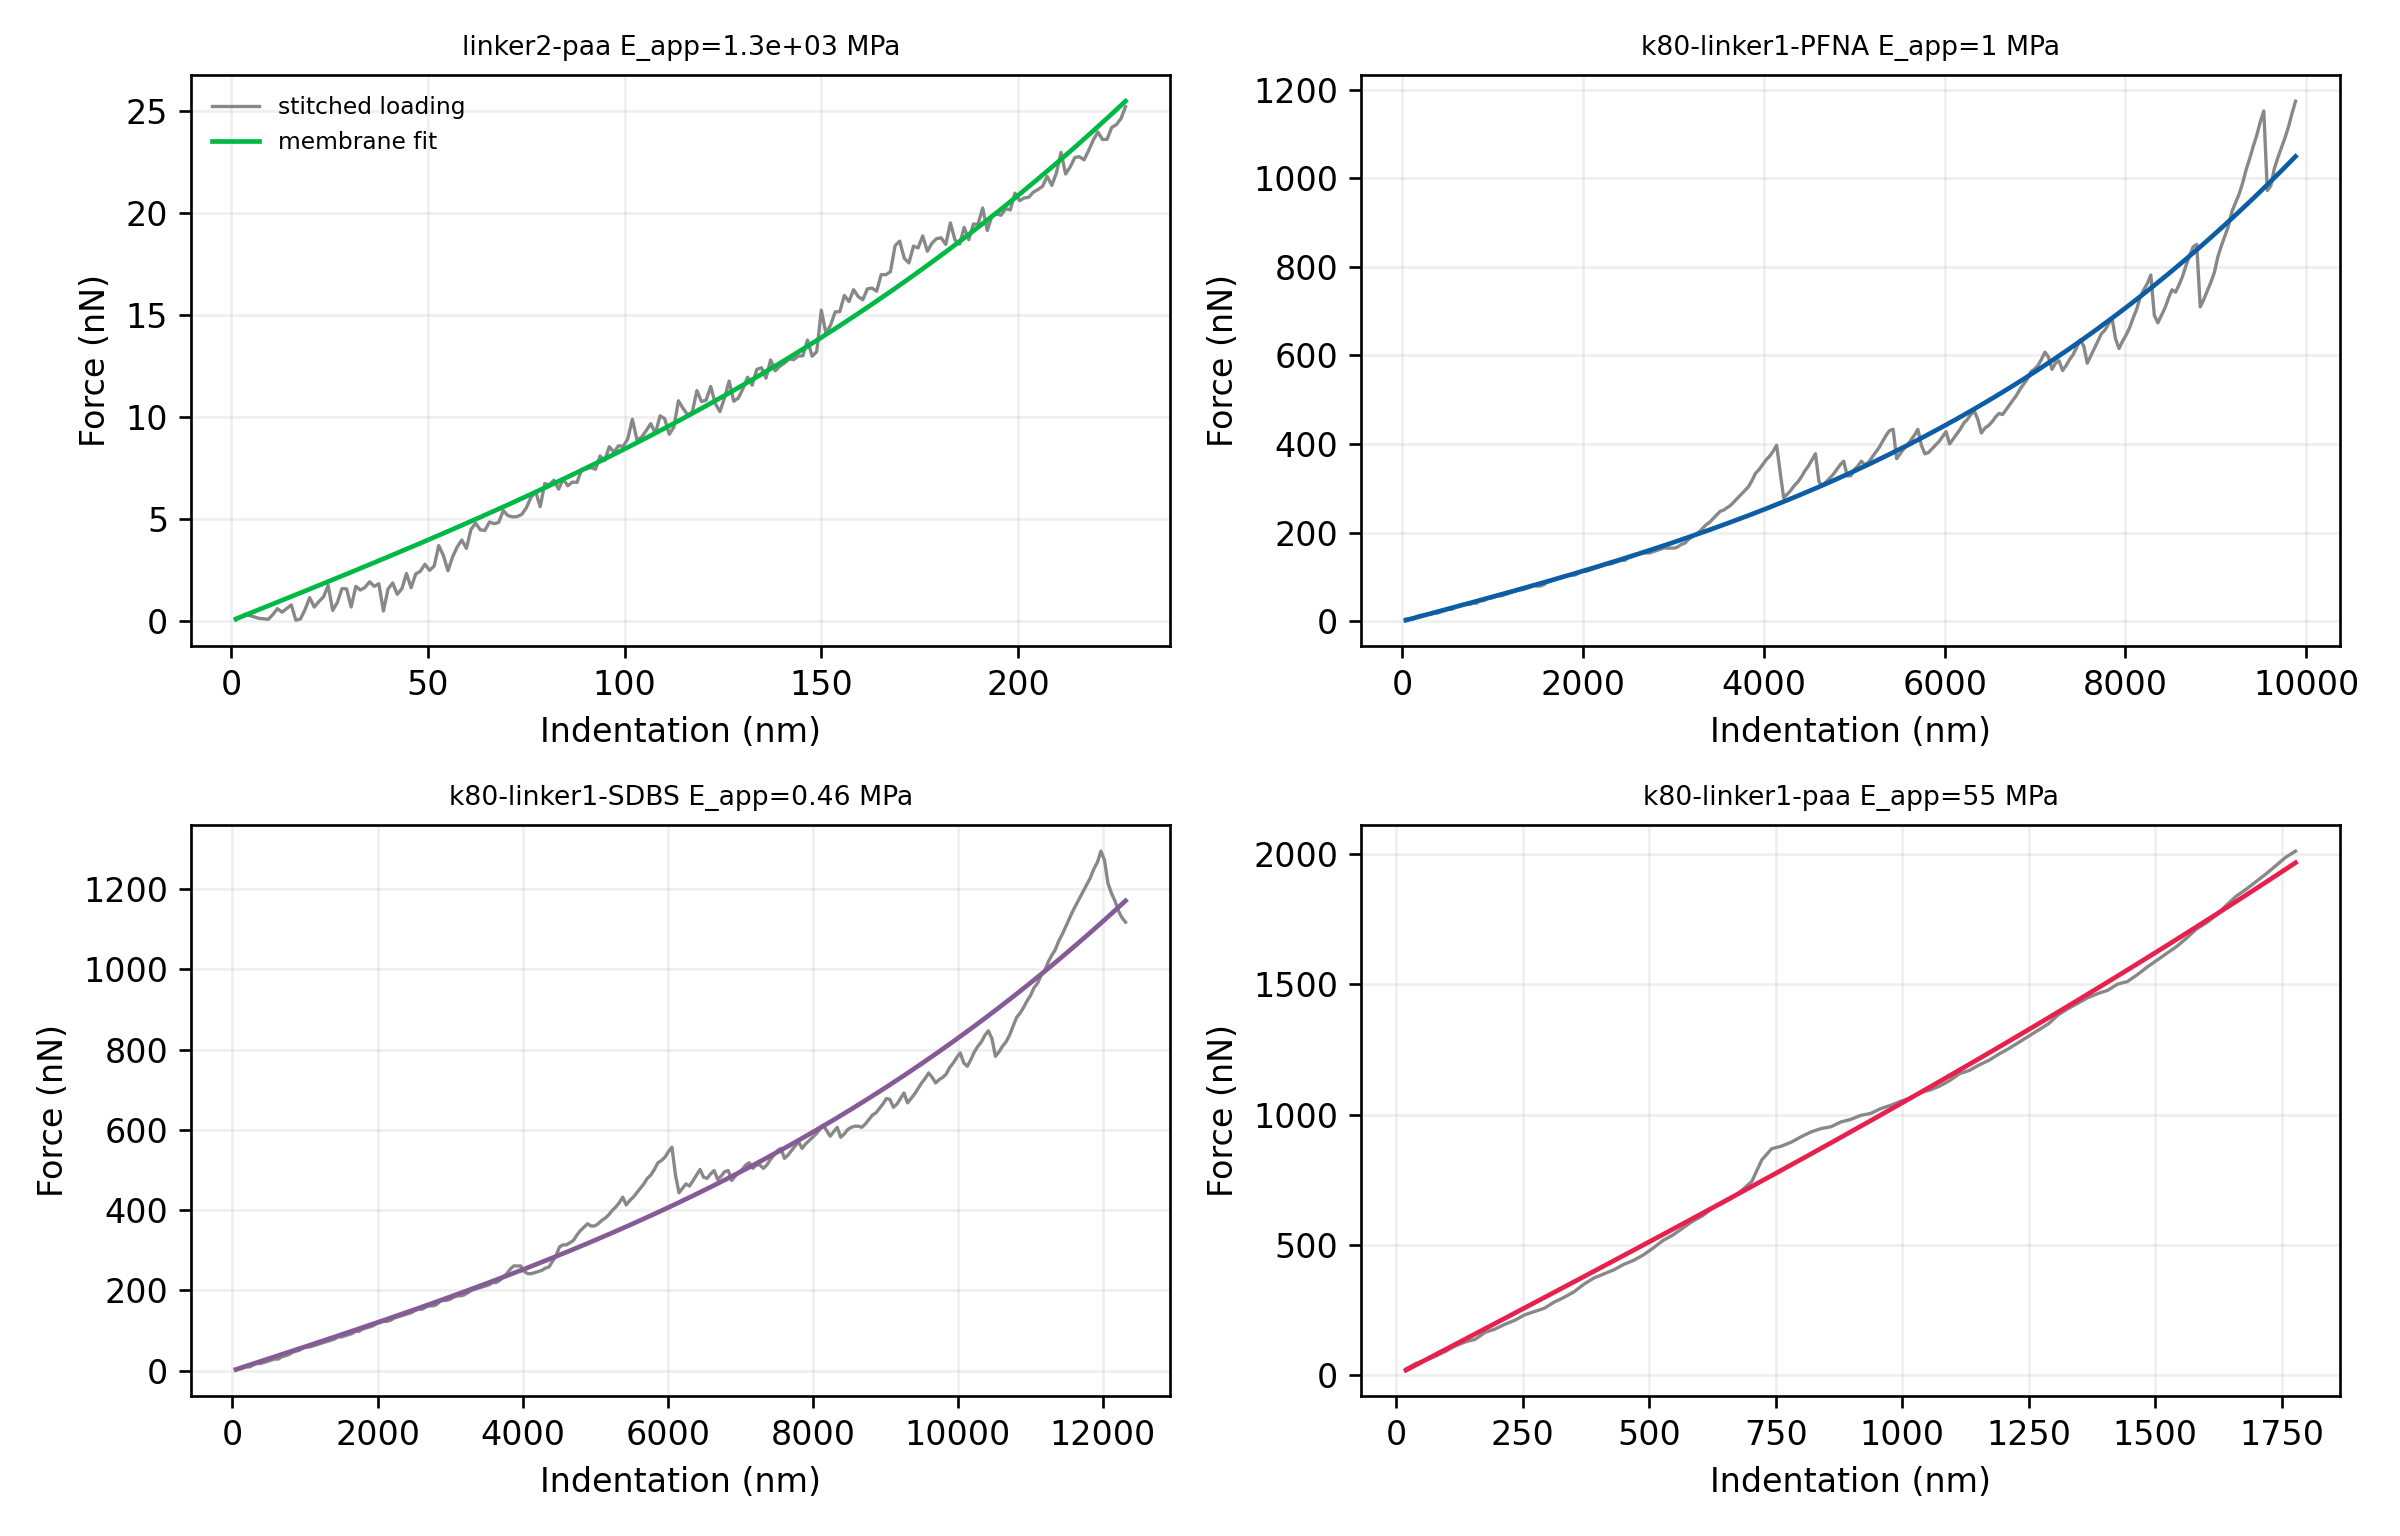
\includegraphics[width=\linewidth]{model_fit_examples.png}
        \caption{代表性 stitched loading 曲线及膜模型拟合。}
        \label{fig:model-fit}
    \end{subfigure}
    \caption{深压入 apparent modulus 分析。所有图均基于 stitched 后的正力 loading 段，JJS、snap-in、pull-off 和 adhesion 信号未纳入力学拟合。组间误差棒优先采用图~\ref{fig:median-iqr} 中的 median+IQR 表示。}
    \label{fig:surfactant-mechanics}
\end{figure}

\begin{table}[htbp]
    \centering
    \caption{不同处理组的深压入表观力学参数。}
    \label{tab:surfactant-mechanics}
    \small
    \setlength{\tabcolsep}{3.5pt}
    \begin{tabular*}{\linewidth}{@{\extracolsep{\fill}}llrrrr}
        \toprule
        日期 & 组别 & 有效曲线 & $E_{\mathrm{app}}$ 50 nm & 高力区刚度 & 拟合 $R^2$ \\
        & & $N$ & median [Q1, Q3], MPa & median [Q1, Q3], N/m & median \\
        \midrule
        20260415 & linker2-PAA & 15 & 1299 [1011, 2184] & 0.170 [0.122, 0.226] & 0.988 \\
        20260416 & k80-linker1-PAA & 11 & 55.1 [2.78, 104] & 1.01 [0.447, 1.38] & 0.994 \\
        20260416 & k80-linker1-PFNA & 6 & 1.52 [0.98, 2.31] & 0.276 [0.201, 0.362] & 0.972 \\
        20260416 & k80-linker1-SDBS & 3 & 0.463 [0.349, 0.584] & 0.161 [0.157, 0.163] & 0.976 \\
        20260416 & k80-linker2-PAA & 0 & -- & -- & -- \\
        \bottomrule
    \end{tabular*}
\end{table}

结果显示，表面活性剂/后处理对悬膜的深压入承载能力具有决定性影响。考虑到 $E_{\mathrm{app}}$ 分布存在长尾，本文以每条曲线为独立统计单元，采用中位数作为中心值，四分位范围（Q1--Q3）作为误差棒。在 20260416 k80 同一钝探针条件下，PAA 处理组的表观膜模量最高，$t=\SI{50}{\nano\meter}$ 假设下中位数为 \SI{55.1}{MPa}，四分位范围为 \SIrange{2.78}{104}{MPa}，高力区表观刚度为 \SI{1.01}{N/m} [\SIrange{0.447}{1.38}{N/m}]；PFNA 组下降到 \SI{1.52}{MPa} [\SIrange{0.98}{2.31}{MPa}]，SDBS 组进一步下降到 \SI{0.463}{MPa} [\SIrange{0.349}{0.584}{MPa}]。由于三组使用相同探针、相近孔径和相同计算模型，该排序比跨日期、跨探针的绝对模量比较更可靠。PAA 组同时具有更高的承载力和更高的 stitched loading 刚度，说明其薄膜在大压入下更能维持连续拉伸网络；相反，PFNA 和 SDBS 组的低模量与低刚度更符合缺陷密度更高、晶粒连接更弱或膜内有效承载路径更少的情形。

20260415 的 linker2-PAA 组表现出更高且更稳定的 GPa 级表观模量：15 条曲线全部通过 QC，$E_{\mathrm{app}}$ 中位数为 \SI{1.30}{GPa}，四分位范围为 \SIrange{1.01}{2.18}{GPa}（$t=\SI{50}{\nano\meter}$）；若取 $t=\SI{80}{\nano\meter}$，中位数为 \SI{0.812}{GPa}。膜模型拟合 $R^2$ 中位数为 0.988。这一结果支持 linker2-PAA 膜具有更连续、更少机械弱点的悬膜网络。不过，20260415 使用 RTESPA-150 小半径探针，而 20260416 使用 DDESP-V2 钝探针，因此 linker2-PAA 与 k80 系列之间不应直接用绝对数值判断材料优劣；更稳妥的表述是：linker2-PAA 在其自身测试条件下显示出最高且最可重复的 apparent membrane modulus，而 k80 内部 PAA 明显优于 PFNA 和 SDBS。

从结构--性能关系上看，表面活性剂可能通过三类途径改变薄膜力学表现。第一，表面活性剂影响成膜过程中的晶粒融合和片层堆积，改变有效承载网络的连续性；第二，表面活性剂残留或相分离会引入软界面、孔洞和局部脱粘位置，使深压入曲线更容易出现滑脱或低刚度响应；第三，亲水/带电基团可能改变 PAA 与 COF/基底之间的界面结合，使大压入下的载荷从局部接触更有效地转移到整张悬膜。当前 AFM 力曲线本身不能直接成像这些缺陷，因此本文将其作为由力学响应反推的候选机制；最终仍需 SEM/TEM、AFM height/phase 或 GIWAXS 等形貌和结构证据来闭合因果链。

与典型材料尺度相比，k80-PAA 的 \SIrange{34}{55}{MPa} 属于软膜到中等聚合物膜范围，显著高于 PDMS 等软弹性体，但低于高强工程聚合物。linker2-PAA 的 \SIrange{0.81}{1.30}{GPa} 已接近低端工程聚合物或部分多孔有机薄膜的量级，但仍低于高度取向的二维聚合物、石墨烯氧化物纸、MoS$_2$ 和 graphene 等高强二维材料。这个数量级关系是合理的：本体系的深压入响应来自多晶/多孔/界面处理后的悬膜网络，缺陷、晶界、膜厚不均和边界夹持都会降低 apparent modulus。因此，本文的关键发现不是达到无缺陷二维晶体的极限强度，而是证明表面活性剂/后处理可以显著调控悬膜的有效承载网络，并使 apparent modulus 跨越超过两个数量级。

\section*{可直接用于正文的结论句}

\begin{sloppypar}
Deep-indentation analysis reveals that surfactant-dependent film formation produces pronounced differences in apparent membrane mechanics. Within the k80 series measured under the same blunt-tip geometry, PAA-treated films exhibit the highest model-dependent apparent modulus and high-force stiffness, whereas PFNA and SDBS lead to much softer loading responses. Together with the robust GPa-level response of linker2-PAA, these results suggest that surfactant-controlled morphology and defect density regulate the continuity of load-bearing pathways in suspended COF films.
\end{sloppypar}

\end{document}
